\hypertarget{funnel-metadynamics-tutorial}{%
\section{Funnel Metadynamics
tutorial}\label{funnel-metadynamics-tutorial}}

Funnel metadynamics (fun-metaD) is a molecular dynamics-based method
that calculates the absolute binding free energy (ABFE) between a small
organic ligand and a protein. It uses an enhanced sampling method called
metadynamics, that speeds up the molecular processes of interest by
periodically adding small amounts of bias. To best separate the bound
and unbound phases, as well as increase the rate of convergence, the
exploration of the ligand in 3D space is limited by funnel-shaped
restraints.

This tutorial aims to describe how to setup and analyse fun-metaD
simulations. The main paper that describes what fun-metaD is by
\href{https://www.pnas.org/content/110/16/6358}{Limogelli \emph{et al}
2013} but in this tutorial I will describe the
\href{https://www.ncbi.nlm.nih.gov/pmc/articles/PMC7467642/}{Rhys
\emph{et al} 2020} and
\href{https://pubs.acs.org/doi/10.1021/acs.jcim.6b00772}{Saleh \emph{et
al} 2017} implementation. The main difference between the two
implementations is the functional form of the funnel restraints: the
original fun-metaD relied on a cone and a cylinder joined to make a
funnel using a step function, while the new implementation uses a single
sigmoid function. The Limogelli implementation also requires the protein
to be realigned with a reference structure to keep the funnel strictly
in place over the binding site, which hurts the performance. The
implementation I will describe here allows the funnel to move with the
protein.

Up to now, one of the biggest drawbacks to using fun-metaD for
large-scale absolute binding free energy (ABFE) calculations was the
difficulty in setting up the simulations. It's hard to know where the
funnel should be defined, how big it needs to be, what each of the
sigmoid function parameters should be set to, along with the chore of
writting PLUMED files, where each protein and ligand system will have
slightly different atom IDs.

BioSimSpace has made this easier, automatically defining the funnel
using abstract features of the protein cavity, assigning the relevant
atom IDs, suggesting reasonable default funnel parameters and allowing
the visualisation of the funnel restraints inside a Jupyter Notebook.
All this leads to a quicker setup and much faster automation of large
ABFE screening campaigns.

By the end of this tutorial you should know: 1. The basics of what
fun-metaD does. 2. How to setup fun-metaD simulations and how to
visualise the funnel restraints. 3. How to analyse the results of a
fun-metaD simulation.

Let's get started.

\hypertarget{part-1---the-theory}{%
\subsection{Part 1 - The Theory}\label{part-1---the-theory}}

Metadynamics is an enhanced sampling method that biases a simulation
along a chosen set of reaction coordinates, or as MetaD practitioners
call them, collective variables (CVs). This bias is deposited at defined
time intervals and takes the shape of a Gaussian potential.
Investigation of drug binding should involve at least one CV, distance
from the drug molecule to the protein, where the distance between them
can be biased, causing the drug to unbind. However, that single distance
is degenerate, meaning many different configurations of the drug in 3D
space will not be described by that single distance. It also involves
the exploration of a very large volume, hindering convergence.

Fun-metaD gets around both of these problems, restricting the
exploration by using funnel-shaped restraints and reducing degeneracy by
using two CVs - `projection' and `extent'. See Figure A.

\begin{figure}
\centering
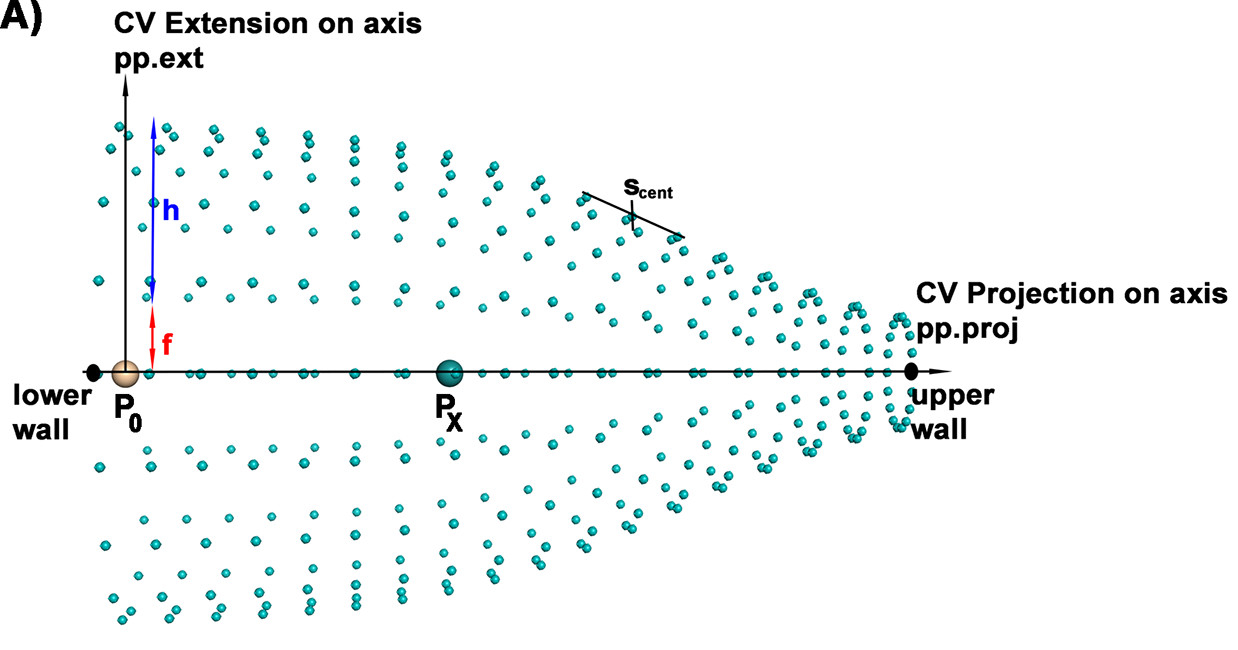
\includegraphics{figures/figure1.jpeg}
\caption{Figure1}
\end{figure}

The restraints that limit the pp.ext CV follow a sigmoid function:

\begin{figure}
\centering
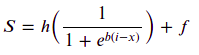
\includegraphics{figures/figure2.png}
\caption{Figure1}
\end{figure}

where, S is the maximal distance from the axis, at pp.proj = i, h is the
`wall\_width', f is the `wall\_buffer', b is the `beta\_cent' (the
steepness at the inflection point), x is the `s\_cent' (the inflection
point as a value of pp.proj). The exploration along the pp.proj is
limited by the `lower\_wall' and `upper\_wall' parameters. The funnel's
radius at the narrow end is equal to `wall\_buffer'. `P0' and `Px' are
the points that define the funnel's vector. From now on I'll refer to
them as p0 and p1, respectively.

It should be obvious that there is still some degeneracy - in the plane
perpendicular to the projection axis. However, this is a good compromise
between having sufficient accuracy for describing the binding of a
ligand and the tolerable simulation slowdown of using only two CVs.

``Where should the funnel point? How big should it be at the base? Do I
need to change the position of the inflexion point? The steepness? How
long should the funnel be?''

There aren't any definite answers to any of these questions. Of course,
the funnel needs to point `out', with the narrow end in the solvent,
away from any protein residues. BSS funnel assignment code addresses
that question pretty well, most of the vectors it picks for defining the
p0 and p1 points are good enough. It's still a good idea to check, by
having a look using BSS' visualisation functionality.

As for picking the parameters for the sigmoid function - the funnel will
need to be smaller than you think. There is usually only one binding
site and the funnel should enclose only it, excluding other protein
features, by setting a small `wall\_width'. This really helps with
convergence by preventing the drug molecule from exploring irrelevant
regions in the free energy surface (FES). Other parameters don't matter
that much and the default numbers will suffice in most situations.

\hypertarget{part-2---setting-up-the-system-visualising-the-funnel-and-preparing-the-fun-metad-simulations}{%
\subsection{Part 2 - Setting up the system, visualising the funnel and
preparing the fun-metaD
simulations}\label{part-2---setting-up-the-system-visualising-the-funnel-and-preparing-the-fun-metad-simulations}}

For this part, open the \texttt{02\_bss-fun-metad-tutorial.ipynb}
notebook.

\hypertarget{part-3---analysis}{%
\subsection{Part 3 - Analysis}\label{part-3---analysis}}

Open the \texttt{03\_bss-fun-metad-analysis.ipynb} notebook.
